\documentclass{beamer}
\usepackage{graphicx}
\usepackage{wrapfig}
\usepackage{setspace}
\usepackage{xcolor}
\usetheme{Madrid}
\usecolortheme{default}

\title[2020MP000]{Video Streaming Platform for open source community}
\subtitle{Project ID:21C131176\\Review -II}
\author[SRM Institute of Science \& Technology]{Group~Members\\RA1711003030131~Kanishk Dixit \\RA1711003030176~Akshay Jain\\ \medskip{Supervised By:\\Mr. Abhishek Singh \\Assistant Professor}}
\institute[]{Department of Computer Science \& Engineering\\Faculty of Engineering \& Technology\\SRM Institute of Science \& Technology}
\logo{\includegraphics[scale=.4]{srm_logo}}
%\author{YYY}
\date{\today}
\begin{document}
	\begin{frame}
		\maketitle
		\date{}
	\end{frame}
	\begin{frame}[t]{Table of Contents} %we can expand the table of contents in more than on frame
		\tableofcontents[sections={1-6}]
	\end{frame}
	\section{Objective}
	\begin{frame}{Objective}
\begin{itemize}
    \item To provide the video streaming experience in a better way over the internet.
    \item To provide a platform for content creators to market there content to the specified users.

    \item  To provide easy accessibility of a specific content to the content consumers.
    \item Create an open source community for this platform.

\end{itemize}	  
	\end{frame}
	\section{Literature Survey}
	\begin{frame}[allowframebreaks]{Literature Survey}
	\begin{itemize}
	 \begin{figure}
		{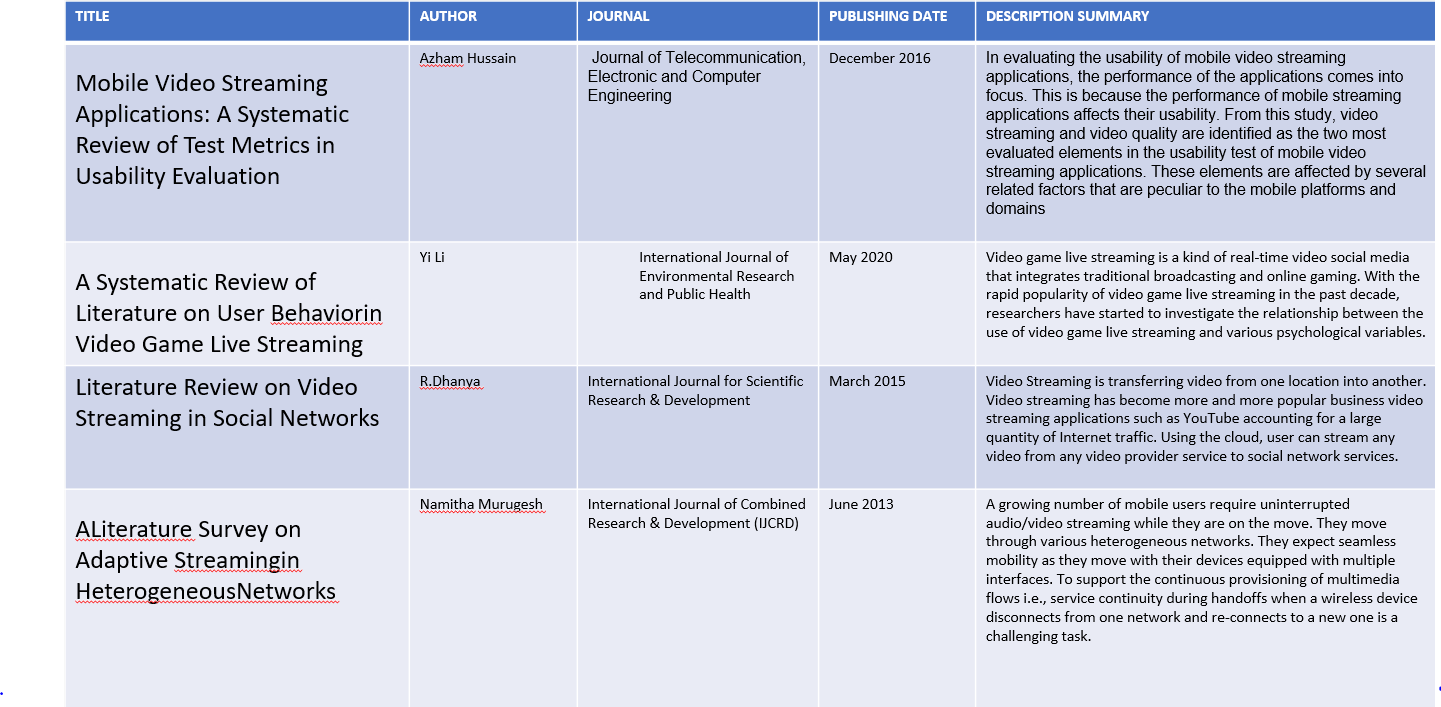
\includegraphics[scale=.37]{ss5.PNG}}
			\caption{Proposed Architecture}
			\label{arch1}
	\end{figure}
		\end{itemize} 
	\end{frame}
\section{Architectural Design For Proposed System}
\begin{frame}[allowframebreaks]{Architectural Design For Proposed System}
    \begin{figure}
		{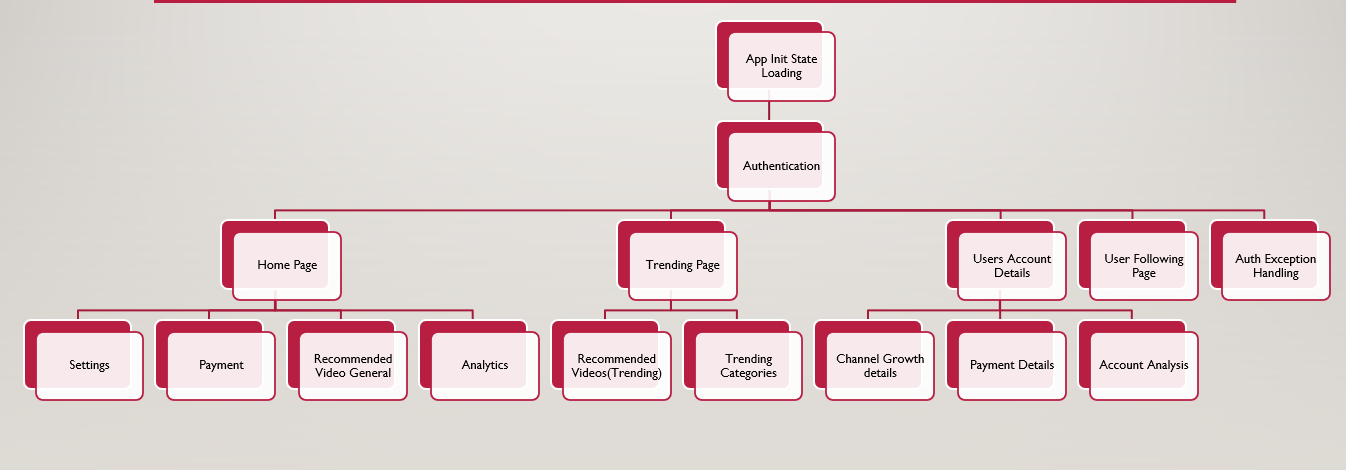
\includegraphics[scale=.4]{arch.PNG}}
			\caption{Proposed Architecture}
			\label{arch1}
	\end{figure}
	\begin{center}
	\textcolor{red}{\textit{Explanation of project Architecture: }}\\
	\begin{itemize}
		\item Init State
		 \begin{itemize}
    \item App will load up into the memory
    
  \end{itemize}
		
		\item  Authentication
 \begin{itemize}
    \item User needs to get authenticated to use the application

     \item There are various ways for authentication like google sign up, facebook signup, phone signup

      \item They will redirect to the Home page after successful Auth. If its gets failed then there will be Auth Exception Handling.

    
  \end{itemize}
		\item  Home Page
 \begin{itemize}
    \item Recommended videos will be shown in the majority of the section.


     \item There will be a app setting, payment ,Analytics section.


      \item Search Bar 


    
  \end{itemize}
		\item Trending Page
\begin{itemize}
    \item Recommended Trending Videos


     \item Trending Categories



     


    
  \end{itemize}
  
  \item User Account Details
\begin{itemize}
    \item Channel Growth Details :- How much channel is growing 
     \item Payment Details:- How money is flowing in the users account 
     \item Account Analysis :- Users Behaviour.


  \end{itemize}
  \item User Following Page.
\begin{itemize}
    \item What kind of channel user is following.
 
   


  \end{itemize}
		\end{itemize}
    \end{center}
\end{frame}
\section{Proposed Software Design}
\begin{frame}[allowframebreaks]{Partial Implementation}
    \begin{figure}
		{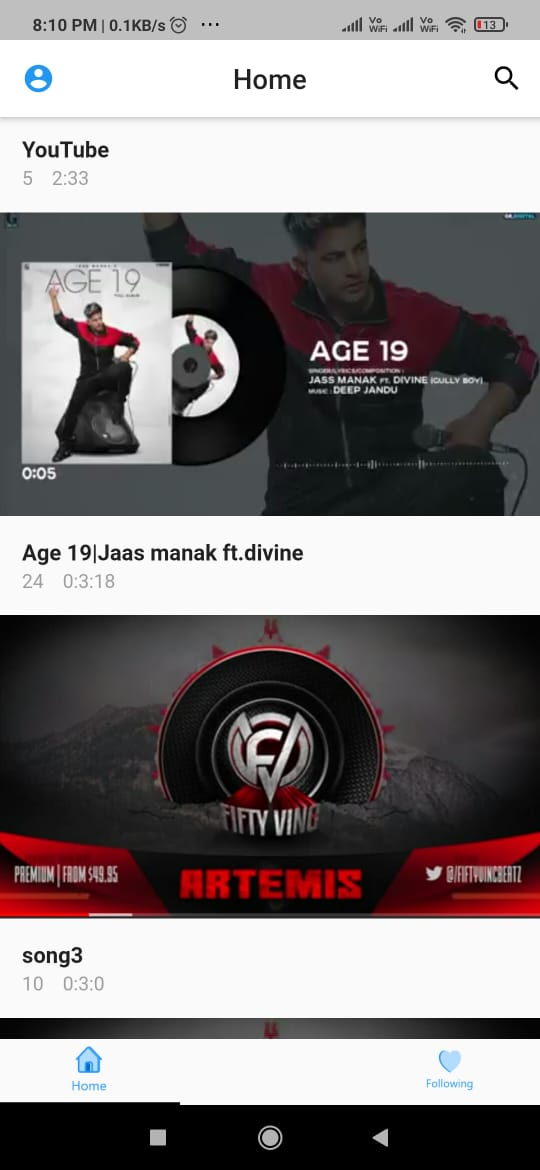
\includegraphics[scale=.11]{ss1.jpeg} 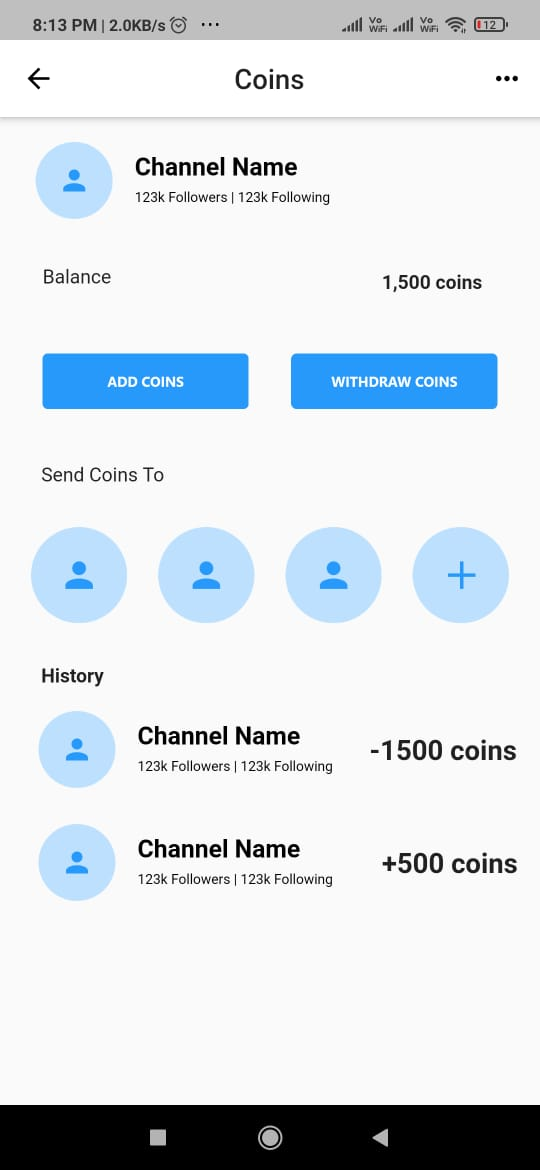
\includegraphics[scale=.11]{ss2.jpeg}
		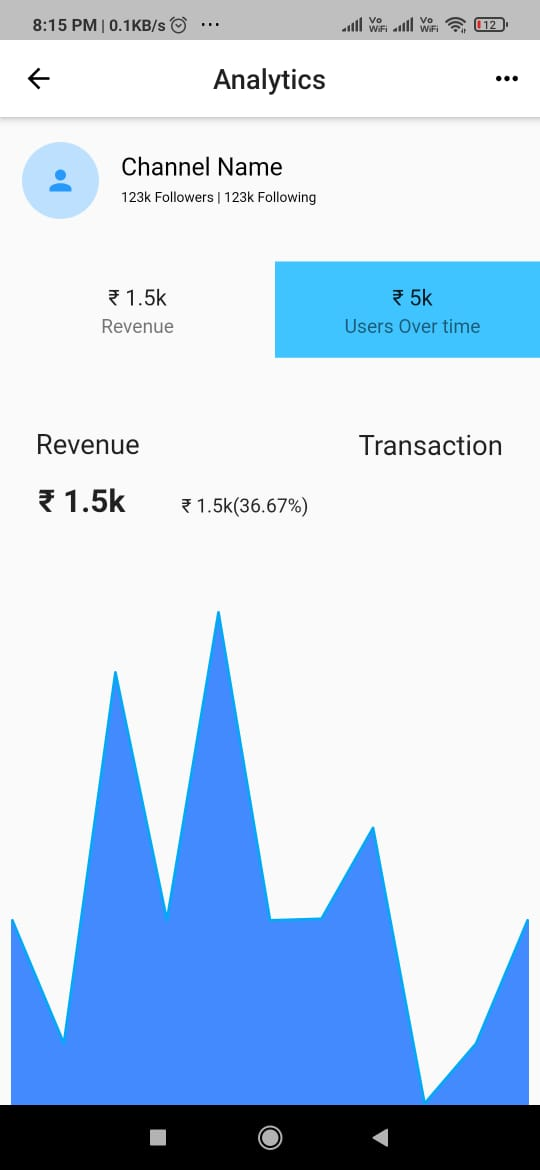
\includegraphics[scale=.11]{ss3.jpeg}
		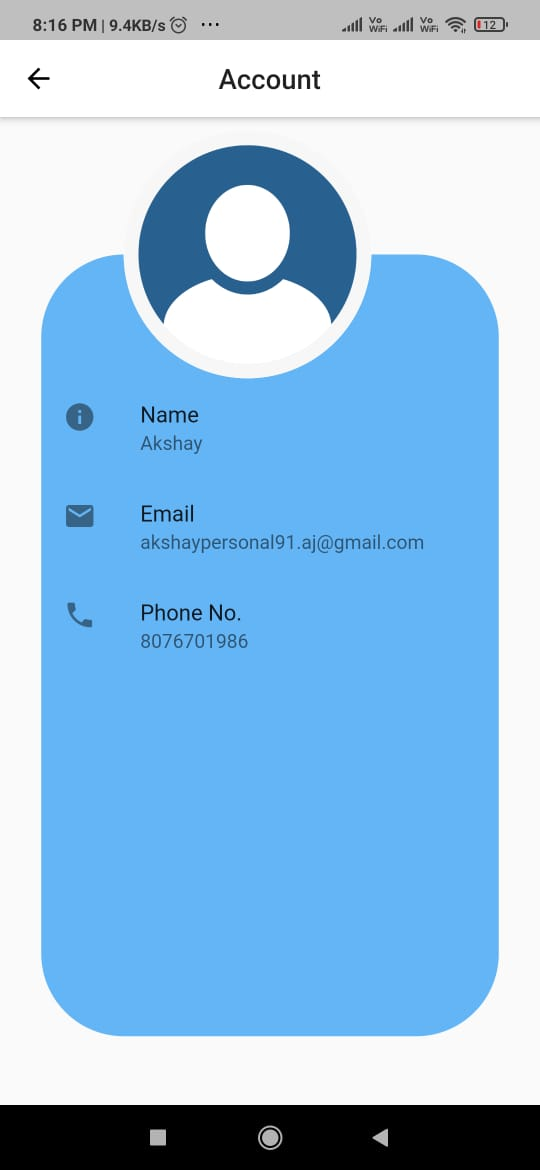
\includegraphics[scale=.11]{ss4.jpeg}
		}
			\caption{Proposed Design}
			\label{arch}
	\end{figure}
	\begin{center}
	\textcolor{red}{\textit{Explanation of Software Design: }}\\
	\begin{itemize}
		\item  On Launching the application, the user will be greeted with Authentication page.
		
		\item After user get logged in the app user will be redirected to home page.
		\item At the home section the content will be show according to the user preferences.
		\item  There will be a trending section where content is recommended to the user according to categories. 
		\end{itemize}
    \end{center}
	
\end{frame}
\section{Techniques to be used}
\begin{frame}[t]{Techniques to be used}
    \begin{center}
	\LARGE
	\textcolor{red}{\textit{Project is Divided into various parts that are executed as follows : }}\\ 
    \end{center}
	\begin{itemize}
		\item Flutter SDK.
		\item Firebase Backend Services(Firebase Auth , Cloud Firestore)

		\item  Android Studio

		\item Machine Learning Algorithms (K Nearest Neighbours most of time) 
		\item Razor Pay API(For Payment Services)
		\item GitHub

	\end{itemize}
	\end{frame}
\section{References}
\begin{frame}[t]{References}
    \begin{center}
        \begin{itemize}
           
            \item Mobile Video Streaming Applications: A Systematic Review of Test Metrics in Usability Evaluation-: Azham Hussain,Journal of Telecommunication, Electronic and Computer Engineering.
           
            \item A Systematic Review of Literature on User Behaviorin Video Game Live Streaming-:Yi Li, International Journal of Environmental Research and Public Health
            
           
            \item Literature Review on Video Streaming in Social Networks :- R.Dhanya,  International Journal for Scientific Research & Development
           
            \item A Literature Survey on Adaptive Streaming in Heterogeneous Networks :- Namitha Murugesh,International Journal of Combined Research & Development (IJCRD)
        \end{itemize}
    \end{center}
\end{frame}


\end{document}